%%%%%%%%%%%%%%%%%%%%%% Props %%%%%%%%%%%%%%%%%%%%%%
\documentclass{article}

\usepackage[french]{babel}
\usepackage[utf8]{inputenc}
\usepackage[T1]{fontenc}
\usepackage{graphicx}
\usepackage{fancyhdr}
\usepackage{eurosym}
\usepackage{color}
\usepackage{soul}
\usepackage{listings}
\usepackage{enumitem}
\usepackage{enumerate}
\usepackage{float}

\pagestyle{fancy}
\lhead{Manuel d'installation}
\chead{Deadly Science}
\rhead{Custos Carceris}



\begin{document}

\tableofcontents

\newpage
\section{Installation}

%%% TODO : Adresse site
Pour installer Deadly Science, il suffit de télécharger l'installateur via le site web du jeu. Ensuite, vous pouvez l'exécuter en double cliquant dessus.

\begin{figure}[H]
	\centering
	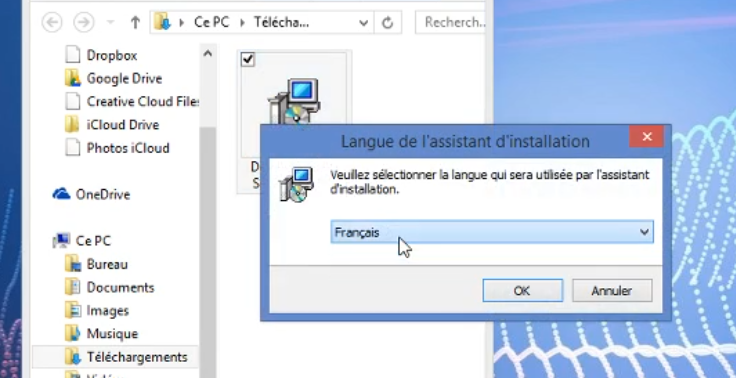
\includegraphics[width=0.49\textwidth]{setup/inst_1.png}
	\caption{Sélection de la langue}
	\label{setup_0}
\end{figure}

Nous voici à la première étape, il suffit de choisir la langue.

\begin{figure}[H]
	\centering
	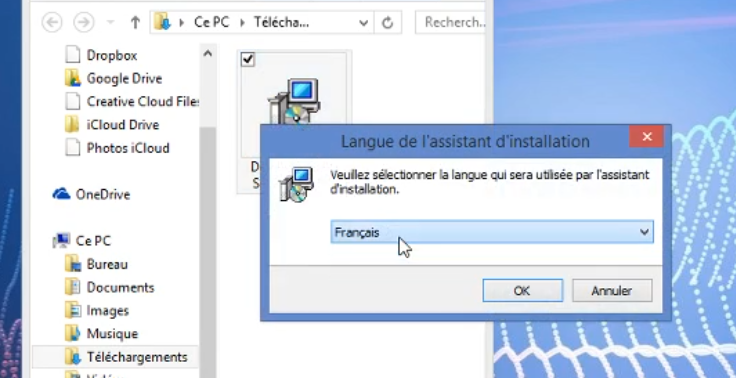
\includegraphics[width=0.49\textwidth]{setup/inst_2.png}
	\caption{Sélection de l'emplacement}
	\label{setup_1}
\end{figure}

Maintenant, il faut choisir où va être installer Deadly Science, nous vous conseillons de laisser les paramètres par défaut pour cette étape.

\begin{figure}[H]
	\centering
	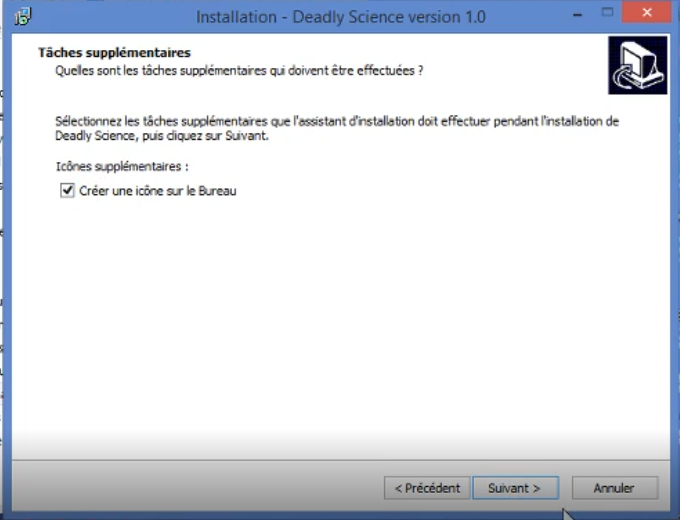
\includegraphics[width=0.49\textwidth]{setup/inst_3.png}
	\caption{Ajout d'un raccourci}
	\label{setup_2}
\end{figure}

Enfin, vous pouvez ajouter un raccourci au jeu sur votre bureau en cliquant sur la case à cocher.
Il ne reste plus qu'à valider puis Deadly Science sera installé et apparaîtra dans le menu démarré.

\newpage
\section{Désinstallation}

Pour désinstaller Deadly Science, il suffit d'aller dans le menu Windows en appuyant sur la touche Windows puis rechercher Deadly Science dans la barre de recherche.
Une fois trouvé, vous pouvez cliquer droit et choisir l'option "désinstaller" ou "uninstall" puis validez votre choix. 

\begin{figure}[H]
	\centering
	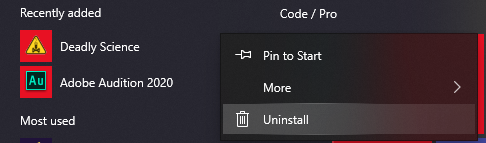
\includegraphics[width=0.49\textwidth]{setup/unins10.png}
	\caption{Désinstallation (Windows 10)}
	\label{setup_3}
\end{figure}

Pour les versions antérieures à Windows 10 il faut trouver le programme "unins000" situé à la racine du dossier Deadly Science, il est situé par défaut à l'emplacement "C:/Users/<Utilisateur>/AppData/Local/Programs/Deadly Science" avec le nom de l'utilisateur à la place de <Utilisateur> puis l'exécuter.

\begin{figure}[H]
	\centering
	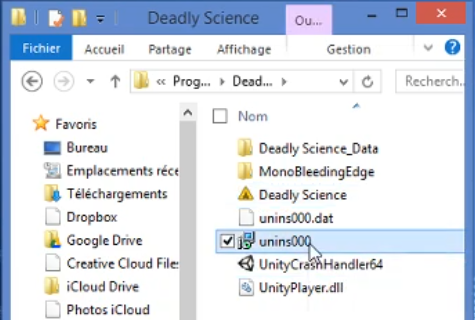
\includegraphics[width=0.49\textwidth]{setup/unins.png}
	\caption{Désinstallation (Windows <10)}
	\label{setup_4}
\end{figure}

\end{document}
